

\begin{figure*}
	\centering
	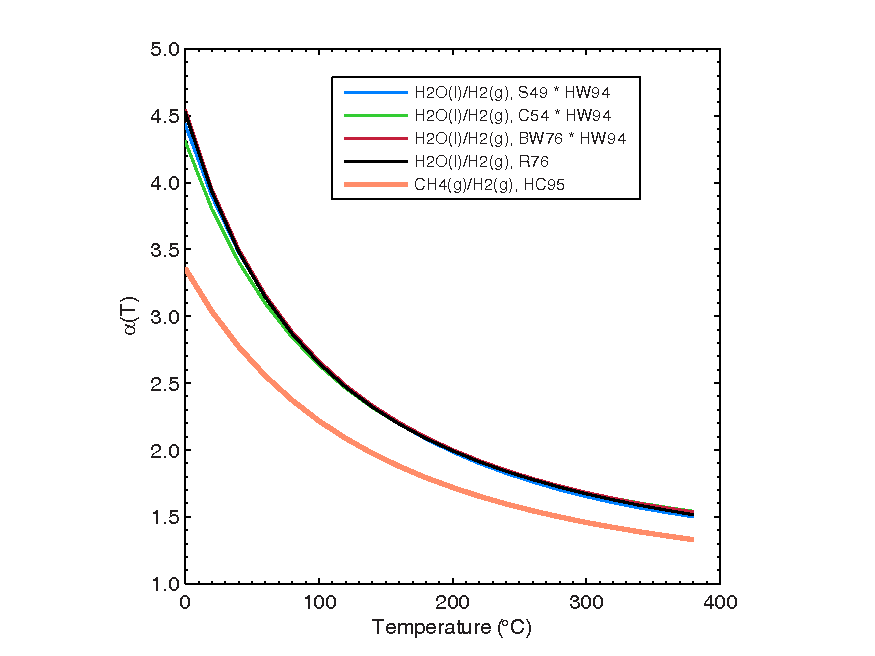
\includegraphics[width=0.8\linewidth]{figures/Fig2.S3}
	\caption[Equilibrium hydrogen isotopic fractionation factors
	for the system H\textsubscript{2}--H\textsubscript{2}O--CH\textsubscript{4}]{Equilibrium hydrogen isotopic fractionation factors
		compiled from experimental and theoretical calibrations. When
	appropriate, calibrations for
	H\textsubscript{2}O(g)/H\textsubscript{2}(g) have been converted using
	the H\textsubscript{2}O(l)/H\textsubscript{2}O(g) calibration from
	\textcite{Horita+Wesolowski_1994_GCA} to derive
	H\textsubscript{2}O(l)/H\textsubscript{2}(g) calibrations. 
	HW94, \textcite{Horita+Wesolowski_1994_GCA}; 
	S49, \textcite{Suess_1949}; 
	C54, \textcite{Cerrai++_1954}; 
	BW76, \textcite{Bardo+Wolfsberg_1976_JPC}; 
	R76, \textcite{Rolston++_1976_JPC};
	HC95, \textcite{Horibe+Craig_1995_GCA}. For any temperature,
	the CH\textsubscript{4}(g)/H\textsubscript{2}O(l) equilibrium
	composition is the ratio of the
	CH\textsubscript{4}(g)/H\textsubscript{2}(g) line (HC95) to a
	H\textsubscript{2}O(l)/H\textsubscript{2}(g) line.}
	\label{fig:2:S3}
\end{figure*}